%%%%%%%%%%%%%%%%%%%%%%%%%%%%%%%%%%%%%%%%%%%%%%%%%%%%%%%%%%%%%%%%%%%%%%
% LaTeX Example: Project Report
%
% Source: http://www.howtotex.com
%
% Feel free to distribute this example, but please keep the referral
% to howtotex.com
% Date: March 2011
%
%%%%%%%%%%%%%%%%%%%%%%%%%%%%%%%%%%%%%%%%%%%%%%%%%%%%%%%%%%%%%%%%%%%%%%
% How to use writeLaTeX:
%
% You edit the source code here on the left, and the preview on the
% right shows you the result within a few seconds.
%
% Bookmark this page and share the URL with your co-authors. They can
% edit at the same time!
%
% You can upload figures, bibliographies, custom classes and
% styles using the files menu.
%
% If you're new to LaTeX, the wikibook is a great place to start:
% http://en.wikibooks.org/wiki/LaTeX
%
%%%%%%%%%%%%%%%%%%%%%%%%%%%%%%%%%%%%%%%%%%%%%%%%%%%%%%%%%%%%%%%%%%%%%%
% Edit the title below to update the display in My Documents
%\title{Project Report}
%
% approach, implementation, results, problems
%
% 1. Introduction
% 1.1. Terms used
% 1.2. Problem definition
% 2. Project specifications
% 2.1. Environment
% 2.2. Modelling
% 3. Implementation
% 3.1. Problems
% 3.2. Known issues
% 4. Results
% 5. Conclusion
% 5.1. Future work
%
% known issues
% future work
%
%%% Preamble
\documentclass[paper=a4, fontsize=12pt]{scrartcl}
\usepackage[T1]{fontenc}
\usepackage{fourier}

\usepackage[english]{babel}                              % English language/hyphenation
\usepackage[protrusion=true,expansion=true]{microtype}
\usepackage{amsmath,amsfonts,amsthm} % Math packages
\usepackage[pdftex]{graphicx}
\usepackage{float}
\usepackage{url}
\usepackage{indentfirst}

\setlength{\parindent}{2em}
\setlength{\parskip}{0.8em}


%%% Custom sectioning
\usepackage{sectsty}
\allsectionsfont{\centering \normalfont\bfseries\scshape}


%%% Custom headers/footers (fancyhdr package)
\usepackage{fancyhdr}
\pagestyle{fancyplain}
\fancyhead{}                      % No page header
\fancyfoot[L]{}                      % Empty
\fancyfoot[C]{}                      % Empty
\fancyfoot[R]{\thepage}                  % Pagenumbering
\renewcommand{\headrulewidth}{0pt}      % Remove header underlines
\renewcommand{\footrulewidth}{0pt}        % Remove footer underlines
\setlength{\headheight}{13.6pt}


%%% Equation and float numbering
\numberwithin{equation}{section}    % Equationnumbering: section.eq#
\numberwithin{figure}{section}      % Figurenumbering: section.fig#
\numberwithin{table}{section}        % Tablenumbering: section.tab#


%%% Maketitle metadata
\newcommand{\horrule}[1]{\rule{\linewidth}{#1}}   % Horizontal rule

\title{
  %\vspace{-1in}
  \usefont{OT1}{bch}{b}{n}
  \normalfont \normalsize \textsc{Technische Universit\"at Dortmund} \\ [25pt]
  \horrule{0.5pt} \\[0.4cm]
  \huge Development of a short-message sharing Web Application in Tapestry5 \\
  \horrule{2pt} \\[0.5cm]
}
\author{
  \normalfont                 \normalsize
    Arthur Xavier Gomes Ribeiro, Rafaella Chaves, Nathan Fabiano\\[-3pt]    \normalsize
    \today
}
\date{}


%%% Begin document
\begin{document}

\maketitle

% 1. INTRODUCTION
\section{Introduction}
In this paper we develop a system used to broadcast short messages between the users.
It is a social network inspired by famous websites and web applications which are currently in trend.
The system developed within this paper is to be considered for academic-only purposes.
It is therefore open source and its source code can be download from \url{http://github.com/arthur-xavier/croak}.

% 1.1. Terms used
\subsection{Terms used}
In this report there are several terms with which the reader might not be familiarized.
And to the fully understanding of the paper, a brief explanation of these terms is understandably needed.
\paragraph{User} A user is an identified and specific person who uses the system described here and can
perform actions within the system and alter its state.
\paragraph{Croak} A croak is a short message (maximal 140 characters) a user can write.
These messages are the core of the system. In the main page of the system the user will be able to
view many diferent croaks.
\paragraph{Follower} A follower is a \emph{User} who follows the user in question and can therefore
see the croaks this user writes.
\paragraph{Friend} A friend is a \emph{User} who either is a \emph{Follower} of the user in question or
a \emph{User} who the user in question follows.

% 1.2. Problem definition
\subsection{Problem definition}
The system designed is the product of a set of actions and restrictions applied to the model.
Below is a detailed description of these.
\begin{enumerate}
  \item Croak a croak
  \begin{enumerate}
    \item The user must be able to write short messages with content up to 140 characters.
    \item These messages must be stored within the database.
    \item The user's friends must be able to see his new message.
  \end{enumerate}
  \item Following list
  \begin{enumerate}
    \item The current user must be allowed to maintain a list of another users whose croaks it follows.
    \item The user must be able to manage this list, begin able to delete or add new friends at will.
  \end{enumerate}
  \item Followers list
  \begin{enumerate}
    \item Alongside the \emph{Following list}, its counterpart, the \emph{Followers list} is a list of another users who follow the current user's croaks.
    \item The user can't but manage this list, as it relies on the other users' behaviour.
  \end{enumerate}
  \item Follow me
  \begin{enumerate}
    \item The user must be able to invite other users to follow his croaks.
  \end{enumerate}
\end{enumerate}

The definition of these parameters was done before anything else, and is the starting point of the development of the system.

% 2. PROJECT SPECIFICATIONS
\pagebreak
\section{Project specifications}
This project is being development as part of the course \textbf{Webtechnologien II}
for the Summer Semester 2015 at the Technische Universit\"at Dortmund.

% 2.1. Environment
\subsection{Environment}
The environment and tools used in the development of the project were quite strict
and could not be chosen freely. On our hands we had a toolset of Java Frameworks and libraries
which, despite not much deep developed, documented or known, have had its own benefits
and use within this project.

The whole set of technologies used are listed below:

\begin{itemize}
  \item Java 8
  \item Maven 4
  \item Tapestry5
  \item JPA
  \item Hibernate
  \item HSQLDB
  \item JAX-RS
  \item Apache Shiro
\end{itemize}

% 2.2. Modelling
\subsection{Modelling}
For the perfect functioning of the system were needed to be created just two Model classes: \textbf{User} and \textbf{Croak}.
A \emph{User} entity has for properties: username; password; first name; last name; email; avatar picture;
and a quotephrase shown in his profile page.
A \emph{Croak} entity has only three properties: text; color; and a \emph{User} author.
A \emph{Invitation} entity has but only two properties: the sender \emph{User}; and the receiver \emph{User}.

Using the conventions stated by Tapestry5, we have divided the system in 9 pages and 2 RESTful resources (one for each entity) used to handle AJAX requests.
The pages used in the system are:
\begin{enumerate}
  \item \textbf{Login} - when the user is not authenticated in the system, this page is shown, either so that it logs in or signs up into the system.
  \item \textbf{Home} - the homepage, where a user can see a short preview of his profile and all the croaks its friends recently wrote.
  \item \textbf{Friends} - this page contains both the \emph{Following list} and the \emph{Followers list} of the current user.
  \item \textbf{Profile} - provides a form where the user can edit and update his profile.
  \item \textbf{Search} - where the user can search for another users or croaks by typing keywords.
  \item \textbf{ViewCroak} - when the user clicks on a croak it is redirected to this page, where it can see the croak alone and bigger.
  \item \textbf{ViewUser} - when the user clicks on a user or a username it is redirected to this page, where it can see the profile and all the croaks written by this user.
  \item \textbf{Logout} - simple action page where the user logs out of the system (no template).
  \item \textbf{Error} - when an error or uncatched exception occurs in the system, this page is shown to the user.
\end{enumerate}

% 3. IMPLEMENTATION
\pagebreak
\section{Implementation}
The implementation of the system was quite difficult and problematic, as there are
not many resources and good documentation for the tools, libraries and frameworks used.
The Tapestry5 framework is also not fully developed and thus creates new small difficulties for developers
as it tries - most of the time successfully - to make it easier.

For the implementation, all the entities were firstly designed along with their respective
RESTful Resources and Data Access Objects (DAOs) interfaces. Then the DAO interfaces were
firstly implemented to store the entities within the application server, using Java Collections.

The Tapestry pages were then created, in order to test the current state of development.

The Hibernate library was then fully integrated in the system as well as the Hibernate
implementation for each DAO interface which now store the entities in a HSQLDB database.

The Apache Shiro authentication and authorization library was then integrated with Tapestry and Hibernate,
and each page and service fully secured.

The Login and Logout pages were finally created and the last bugs corrected.

The Invitation mechanism was implement after the system was already fully functional.

% 3.1. Details
\subsection{Details}
The tapestry-routing library (by Tynamo) was used in order to provide better URLs for the system,
as seen in the user profile URLs (e.g. /@username).

The system provides two DAO implementations for each model class: one using Java Maps
and the other one using Hibernate. This was done in order to provide an easier way
of implementing the system in parts - testing the system functions and specifications
before integrating with Hibernate and a database. This also makes it possible to
extend the system in the future, as it exposes generic DAO interfaces for the entities.

The frontend of the application was developed following the principles stated in
Google's Material Design Guidelines (\url{http://www.google.com/design/spec}).
This was done so that the application would suit better modern users, attract them
with beautiful visuals and work well in mobile devices.

\pagebreak

% 3.2. Problems
\subsection{Problems}
During the development we encountered some problems which might be worth reporting.

Tapestry5, showing one more time that, despite the version number, is not mature enough
to compete with another vanguard Java Frameworks for web development, conflicts with
some JavaScript frontend frameworks such as jQuery. This happens because Tapestry5 makes
use of Prototype, another JavaScript frontend framework which uses the same global variable
as jQuery. This problem could be easily solved by guarding this global variable within the
Tapestry dependencies and JavaScript files in a protected scope.

The libraries developed by Tynamo (such as tynamo-routing and tynamo-security used in this project)
must be correctly labeled as for compatibility with Tapestry5 versions, as they are not backward compatibles.
We had a big problem figuring out that the latest version of tynamo-routing does not work
with Tapestry 5.3.8, as it does not generate any errors or clues to the fact.

Another problem with which we had to deal during the development was the filtering system
used by the tynamo-security library which implements Apache Shiro for Tapestry5.
As the login page of the application contains two Tapestry forms (which generate two diferent
response/action URLs), the tynamo-security filtering system (authc) was not able to deal well with
forwarding requests after the login. We went around this problem by leaving the \emph{authc} filter
and using a simple \emph{user} filter for protected pages and adding an automatic redirection function
in the Error page when it shows authentication errors.

% 3.3. Known issues
\subsection{Known issues}
The page for profile edition lacks validations which could be easily developed by adding
Tapestry5 annotations over the properties for the form fields in page's server-side class.

As for the database, our passwords are stored in plain text, as the application is not meant to be used in
Production environment. In order to facilitate the testing and development, the Sha-256 Hash which was used
at first to store the passwords for the users was replaced by simple plain text storage. This change can
but be reversed by uncommenting both lines at the following files:
src/com/com/croak/dao/hibernate/CroakDAOHibernateImpl.java:44 and
src/com/com/croak/security/UserRealm.java:24.

And last but not least, the system lacks and administrator user. That means it is
still not possible to administrate the system (users and croaks) via the own application.
The system administrator would need to make use of the REST API.


% 4. RESULTS
\pagebreak
\section{Results}
The final results of the development process are to be shown in this section.
Quite satisfactory, following all of the project specifications (but the \emph{Follow me} feature),
the application presents no errors or runtime exceptions when executing any function.
It is known to be fully functional and working well also in mobile devices.

The following screenshots intend to show the application's final design and features.

\subsection{Login page}
\begin{figure}[H]
  \begin{center}
    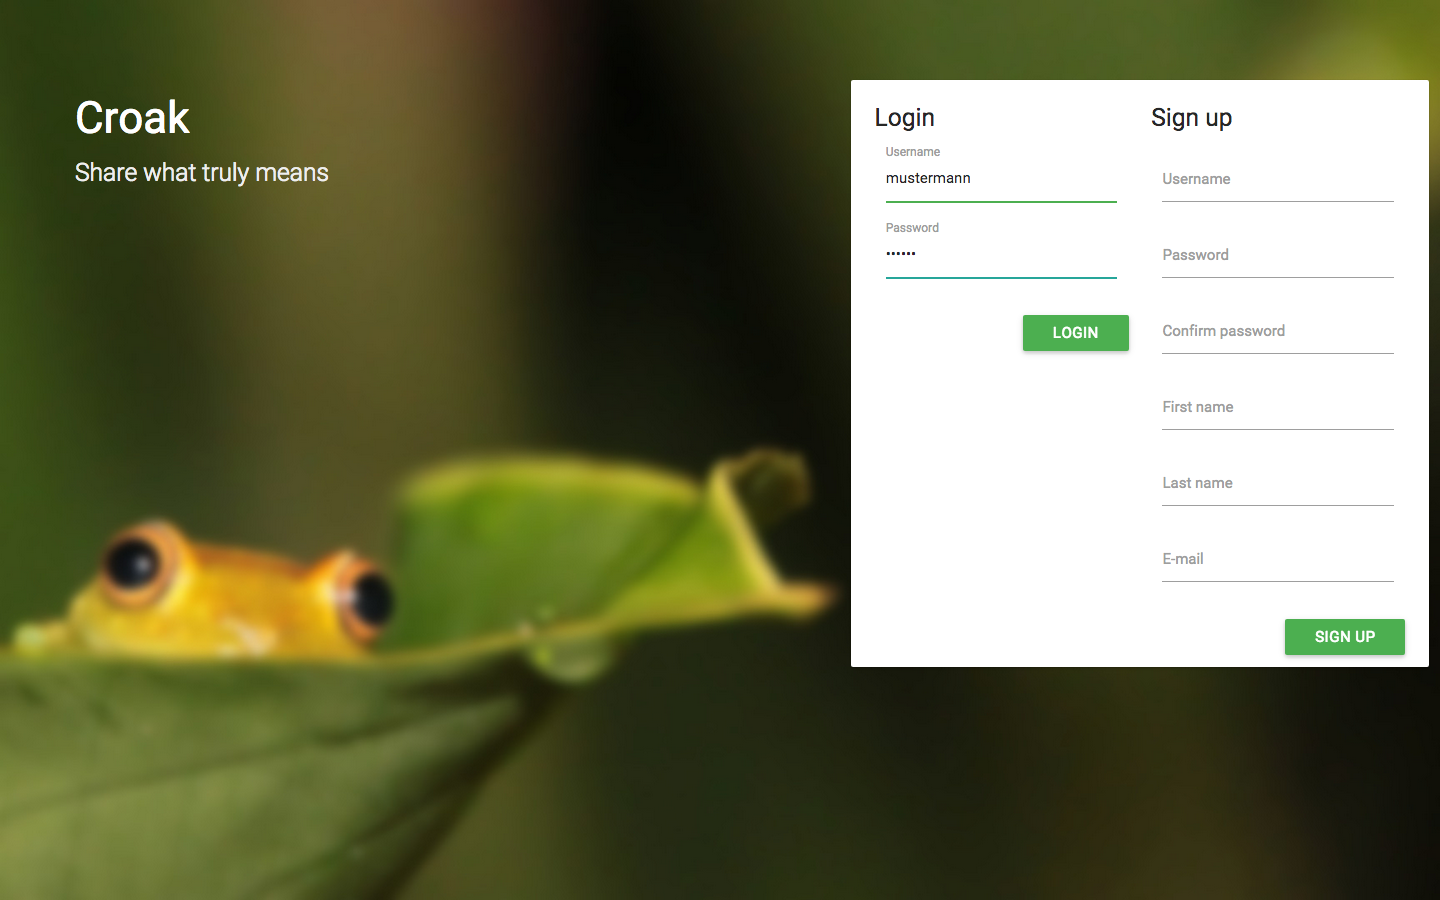
\includegraphics[width=0.75\textwidth]{screenshots/login}
  \end{center}
  \caption{Screenshot of the login page}
\end{figure}

Containing two forms - one for login and the other for signing up -, this page was
quite complicated in development for the difficulties in integrating Apache Shiro's
filtering (authc) functions with the system URLs. As the login page itself contains two Tapestry5 forms,
and is also target of redirection when the user tries to access any page of the system
when not authenticated, the Apache Shiro framework does not integrate quite well with the
Tapestry5 way of routing the forms' actions.

Tapestry5 validations were added to this page to prevent the users from registering with invalid information.

\subsection{Home page}
\begin{figure}[H]
  \begin{center}
    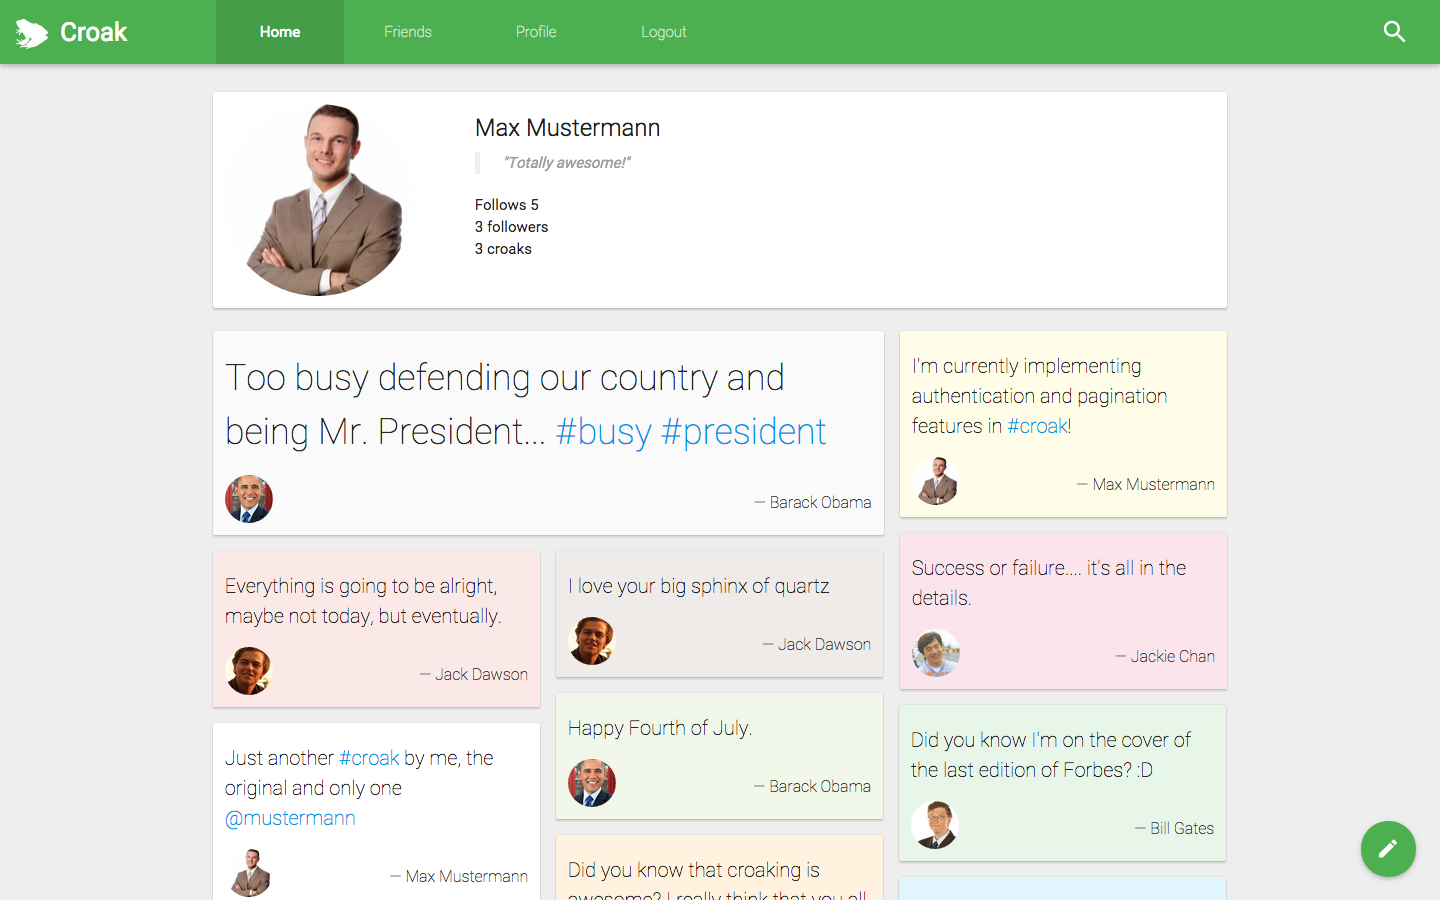
\includegraphics[width=0.75\textwidth]{screenshots/home}
  \end{center}
  \caption{Screenshot of the home page}
\end{figure}

The home page is obviously the center of the system. Here the user has access to the latest
croaks written by the ones he follows. He has also a short overview of his profile
and some statistics about himself. By clicking at the button in the bottom right corner
of the screen (the button is present in all the pages), the user is shown a form for writing a croak.

\subsection{Friends page}
\begin{figure}[H]
  \begin{center}
    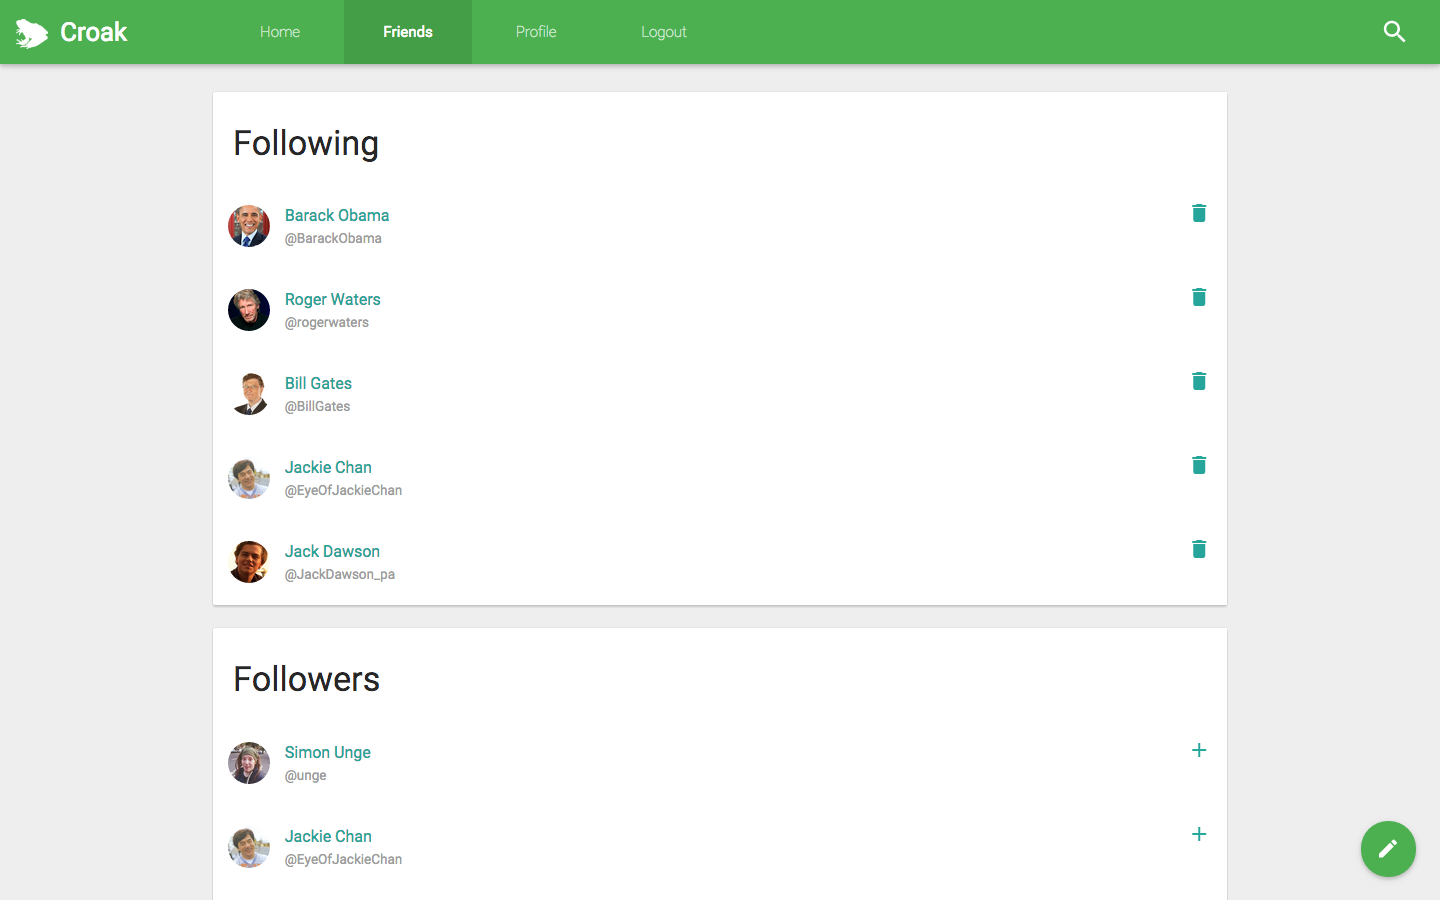
\includegraphics[width=0.75\textwidth]{screenshots/friends}
  \end{center}
  \caption{Screenshot of the friends page}
\end{figure}

In the friends page, the user can view, select, add or remove friends from his \emph{Following list}
or \emph{Followers list}. Shortcut buttons for adding or removing someone from the lists
are provided in the right side of the list after each element, so that the user doesn't
need to go to a friend's profile and click another button to follow or unfollow this person.

\subsection{View user page}
\begin{figure}[H]
  \begin{center}
    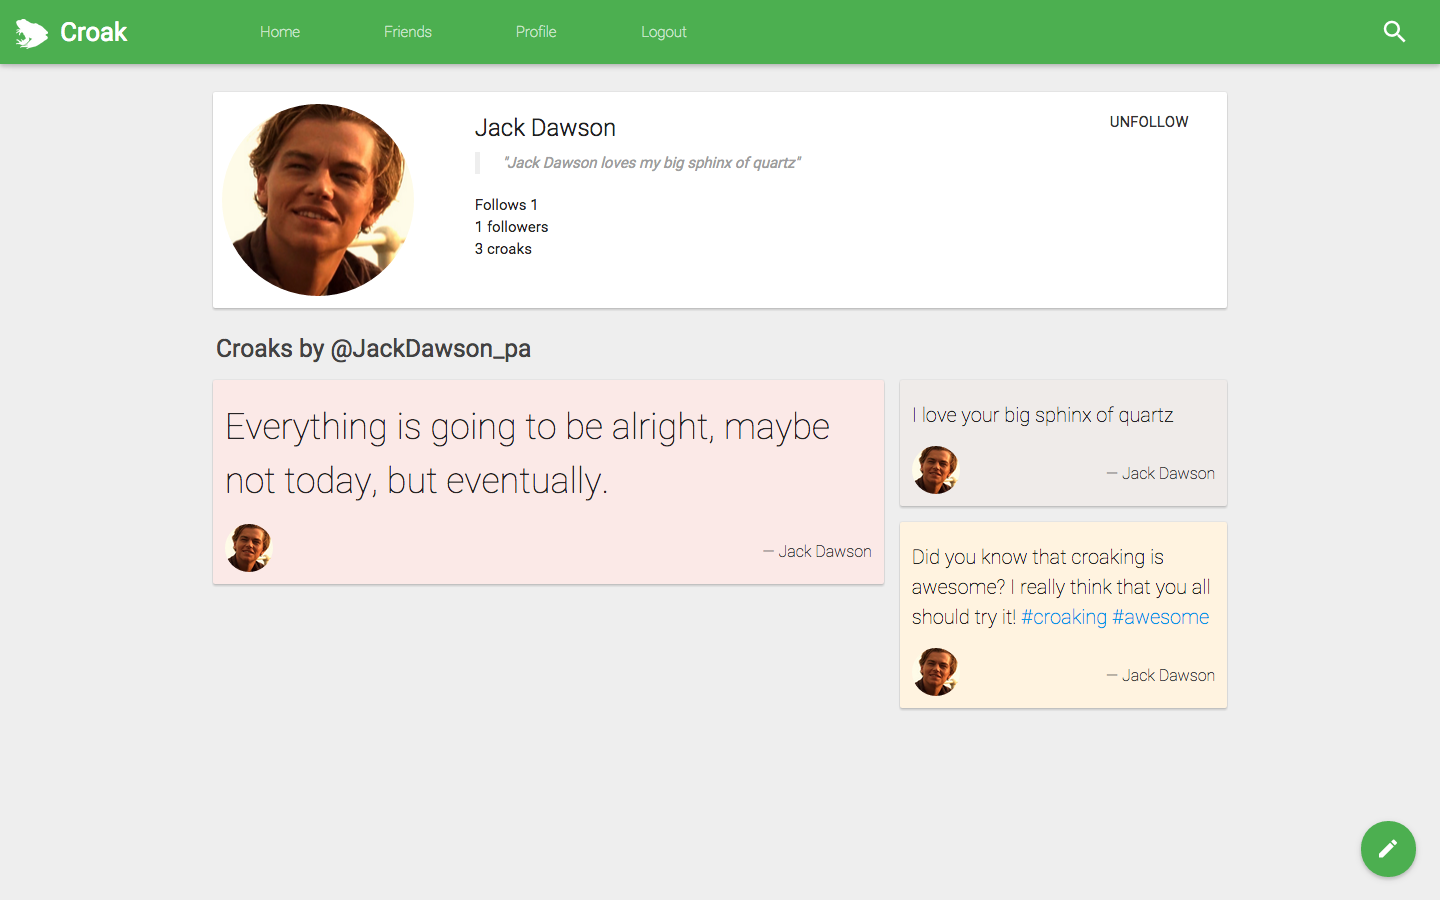
\includegraphics[width=0.75\textwidth]{screenshots/viewuser}
  \end{center}
  \caption{Screenshot of the view user page}
\end{figure}

In this page the user can view informations about another user. Just as in the home page
the user has access to the same informations displayed there but for another user.
He can also click a button in the top right corner of the information card to follow or unfollow
this another user.

Below the information card, the user can view all the croaks posted by the another user in question.

\subsection{Profile page}
\begin{figure}[H]
  \begin{center}
    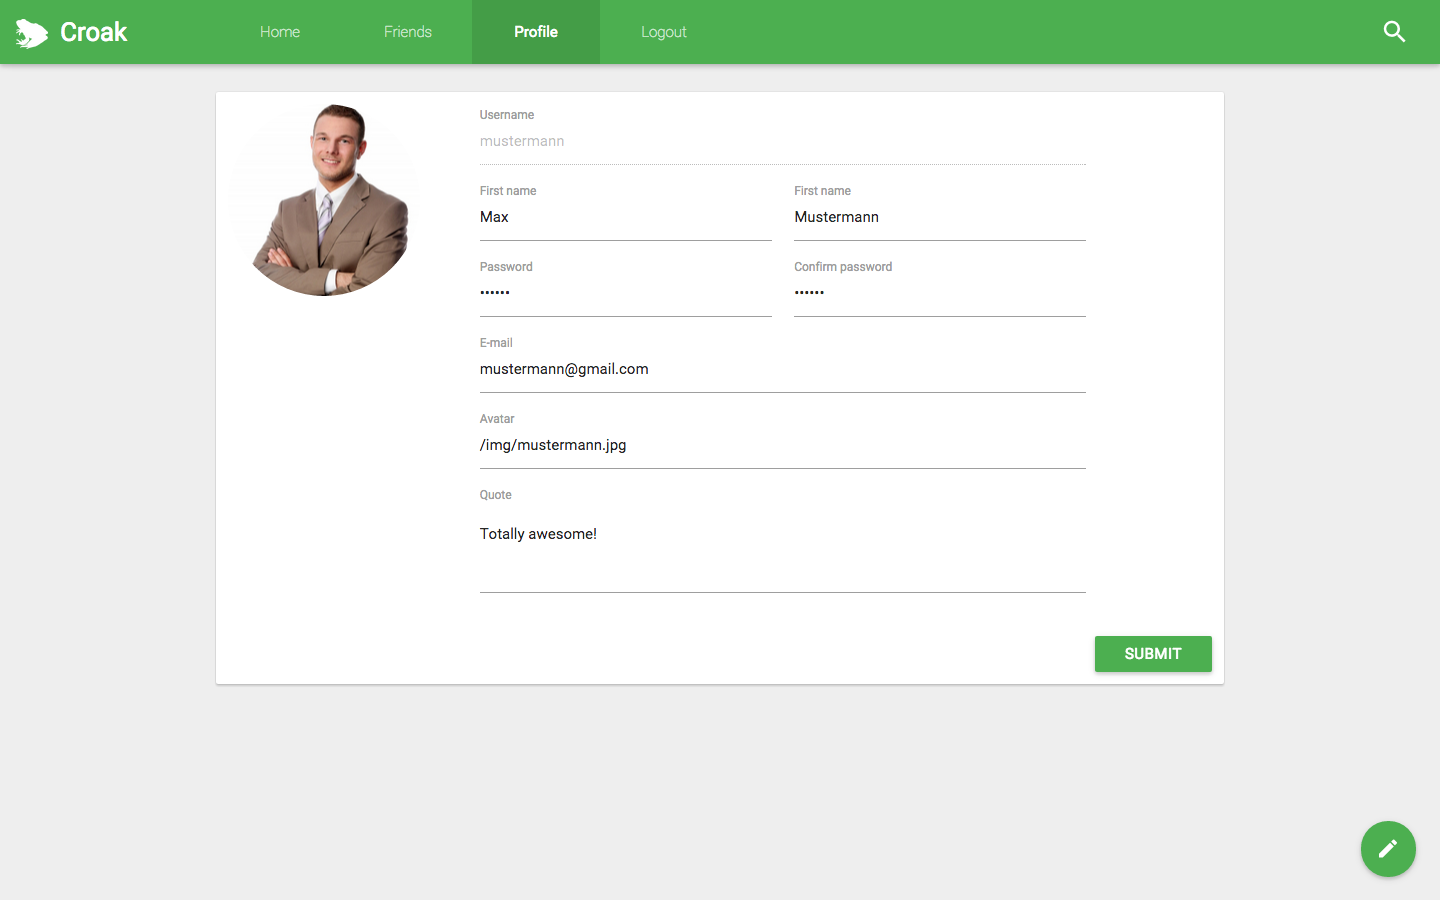
\includegraphics[width=0.75\textwidth]{screenshots/profile}
  \end{center}
  \caption{Screenshot of the profile page}
\end{figure}

Last page shown in this report, the profile page contains a form where the user
can view and edit informations regarding his own profile.

% 5. CONCLUSION
\pagebreak
\section{Conclusion}
Tapestry5, despite being still not fully developed, well-known nor well-documented,
provides really what it promises: an easy-to-use environment Rapid Application Development.
The choice for this framework in order to create a Java based simple/prototype Web Application
is, because of that, remarkable.

Having more time for the development, guidance and organization (both in the development
team itself and from the Tapestry5 developers), this project could have been fully
developed up to the final stage of a refined, production ready industrial application.

Nevertheless the results from the project are quite exciting, showing that, although the team
does not master the environment, a well developed application came out of it.

% 5.1. Future work
\subsection{Future work}
A better password storage algorithm is also a possibility for future work in this application.
It is much more a feature missing in the system than a future work idea, because when it comes
to security guarantees, this is a must in any modern web service.

User authorizations and roles, such as a super user (admin user) would be likely to be
implemented in future versions, as this provides an easier way of managing the system.

Still in the security topic, prevention against SQL Injection can easily be implemented
in future versions by making use of some well developed Java libraries for security.
Using these libraries it would also be easy to add further security improvements,
such as captchas in the Login page.

Another feature which would come right in hand of the users is the ability to upload your own avatar pictures
instead of referencing and external image by its URL in the profile. This was not done here in order to simplify the development, as it
is considerably complicated to implement uploads and server-side storage in Tapestry5.

And a last feature thought for implementation in future versions is a simple AJAX-based
pagination for the viewing of croaks, both in the Home page and in the View User page.
This is not only a nice feature, but would also be needed as the system grows due to
a high count of users and messages.

%%% End document
\end{document}
